% !TeX root = ../../Book2.tex
% 纲要标题：### 17.2 次水平集的变化
% 纲要位置：几何学计划纲要.md，第 1666 行。
% 正文状态：初稿；尚未正式审核。

% 纲要内容开始
% 
% * 无临界区间的梯度变形
% * 跨越单个临界值的局部模型
% * 把手附着映射与指标
% * 从把手到胞腔同伦类型
% 
% 纲要内容结束

\section{次水平集的变化}
\label{g2:sec:1702}

把一个函数的高度从低向高扫描，得到一族不断增大的区域。Morse 引理描述了临界点附近的高度，却还没有说明这个小区域怎样接到已经出现的部分。本节把两件事连接起来：无临界点处用流搬运等高面，临界点附近则直接放入一个有厚度的圆盘。它的厚度保留光滑流形结构，中心圆盘负责改变同伦型。

\subsection{无临界区间的梯度变形}
\label{g2:subsec:1702:01}
记 \(M^a=f^{-1}(( -\infty,a])\)，称为 \(f\) 的\term[cishuipingji]{次水平集}[sublevel set]。若 \(a\) 是正则值且 \(f^{-1}(a)\) 位于 \(M\) 内部，则正则水平集定理给出 \(M^a\) 的新边界 \(f^{-1}(a)\)。在局部坐标中，\(f-a\) 本身就是横向坐标，因而次水平条件成为一个半空间条件。

\begin{proposition}\label{g2:prop:morse-regular-band}
	设 \(M\) 为光滑流形，\(f:M\to\mathbb R\) 光滑，\(a<b\)，且 \(f^{-1}([a,b])\) 是位于 \(M\) 内部的紧集，其中没有临界点。则
	\[
		f^{-1}([a,b])\cong f^{-1}(a)\times[a,b]
	\]
	的微分同胚可取为使 \(f\) 对应第二投影；\(M^a\hookrightarrow M^b\) 是强形变收缩的包含映射，\(M^a\) 与 \(M^b\) 也微分同胚。
\end{proposition}
\begin{proof}
	选光滑 Riemann 度量。由于 \(\mathrm{d}f\ne0\)，向量场
	\[
		Y=\frac{\operatorname{grad}f}{|\operatorname{grad}f|^2}
	\]
	在闭带的某邻域有定义，且 \(Yf=1\)。用紧支截断将它延拓到 \(M\) 上，保持闭带附近的表达。第一卷第13章第1节的光滑流定理及第2节的紧支完备性说明，这个紧支向量场的流 \(\Phi_t\) 对全部时间存在；轨道留在闭带期间满足 \(f(\Phi_t(x))=f(x)+t\)。于是
	\[
		(z,t)\longmapsto\Phi_{t-a}(z),\qquad
		x\longmapsto\bigl(\Phi_{a-f(x)}(x),f(x)\bigr)
	\]
	互为光滑逆。这也解释了紧性的作用：所需时间内的轨道不会在空间中逃走。

	在 \(M^b\) 上令
	\[
		R_s(x)=
		\begin{cases}
			x,&f(x)\le a,\\
			\Phi_{-s(f(x)-a)}(x),&a\le f(x)\le b,
		\end{cases}
		\qquad 0\le s\le1.
	\]
	两式在 \(f=a\) 处一致，给出连续同伦，且逐点固定 \(M^a\)。当 \(s=1\) 时，整个上方闭带落到 \(f^{-1}(a)\)，故得到强形变收缩。

	为得到微分同胚，取 \(a\) 以下一个足够薄的无临界领带；它由闭带的紧性及 \(\mathrm{d}f\ne0\) 延伸得到。在乘积坐标中，用一个光滑严格递增的区间微分同胚把 \([a-\delta,b]\) 压到 \([a-\delta,a]\)，并使它在左端附近为恒等。与更低处的恒等映射拼接，即得 \(M^b\cong M^a\)。这里的压缩移动了边界；前一个强形变收缩则只要求连续，并固定整个旧区域。
\end{proof}

\begin{example}
	在 \(M=\mathbb R^2\setminus\{(0,0)\}\) 上取 \(f(x,y)=x\)。它处处无临界点，但 \(f^{-1}(0)\) 有两个连通分支，其他水平集都是一条直线。\(M^{-1}\) 可缩，而 \(M^1\) 绕缺失的原点有一个不可缩圆周。闭带不紧，正是上面命题无法使用的条件：穿过原点的水平搬运会离开 \(M\)。
\end{example}

\subsection{跨越单个临界值的局部模型}
\label{g2:subsec:1702:02}
现在设临界点 \(p\) 的指标为 \(\lambda\)，写 \(\mu=n-\lambda\)。由\cref{g2:thm:morse-lemma}，可在 \(p\) 附近选坐标 \((u,v)\in\mathbb R^\lambda\times\mathbb R^\mu\)，使
\begin{equation}\label{g2:eq:morse-local-handle-model}
	f(u,v)=c-|u|^2+|v|^2,\qquad c=f(p).
\end{equation}
负方向 \(u\) 在离开临界点时降低高度，正方向 \(v\) 提供横向厚度。选充分小的 \(\varepsilon>0\) 和 \(r>0\)，满足 \(r^2<\varepsilon\)，并使下面的闭集全落在坐标域中：
\[
	H=\bigl\{(u,v):|v|\le r,\ |u|^2\le\varepsilon+|v|^2\bigr\}.
\]
它有一个明确的乘积参数化
\begin{equation}\label{g2:eq:morse-handle-parametrization}
	\Phi:D^\lambda\times D^\mu\longrightarrow H,
	\qquad
	\Phi(x,w)=\bigl(\sqrt{\varepsilon+r^2|w|^2}\,x,rw\bigr).
\end{equation}
缩放因子严格为正，故这是带角流形之间的微分同胚。代入高度可见
\[
	f\circ\Phi
	=c+r^2|w|^2-(\varepsilon+r^2|w|^2)|x|^2.
\]
因此 \(H\subset M^{c+\varepsilon}\)，且
\begin{equation}\label{g2:eq:morse-handle-attaching-face}
	H\cap M^{c-\varepsilon}
	=\Phi(S^{\lambda-1}\times D^\mu)
	\subset f^{-1}(c-\varepsilon).
\end{equation}
新块只沿第一因子的边界贴到旧区域上；它的其余内部点都在旧水平以上。\(\lambda=0\) 时约定 \(S^{-1}=\varnothing\)，新块与旧区域不相交；\(\mu=0\) 时新块是整个 \(n\) 维圆盘，其全部边界都被附着。

\begin{figure}[htbp]
	\centering
	% !TeX root = ../Book2.tex
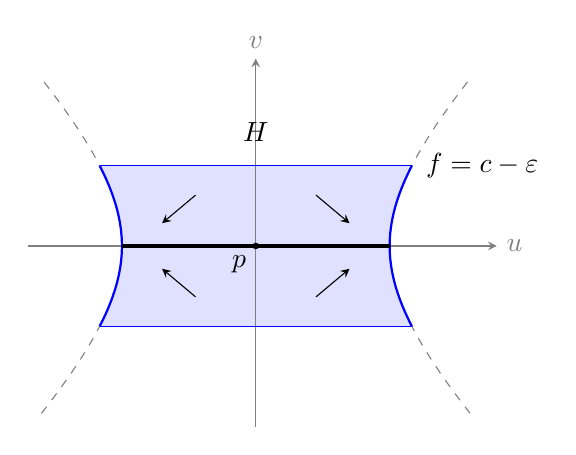
\begin{tikzpicture}[scale=1.7,>=stealth]
	\fill[blue!12] plot[domain=-.6:.6,samples=40] ({sqrt(1+\x*\x)},\x) -- plot[domain=.6:-.6,samples=40] ({-sqrt(1+\x*\x)},\x) -- cycle;
	\draw[->,gray] (-1.7,0)--(1.8,0) node[right] {\(u\)};
	\draw[->,gray] (0,-1.35)--(0,1.4) node[above] {\(v\)};
	\draw[dashed,gray] plot[domain=-1.25:1.25,samples=50] ({sqrt(1+\x*\x)},\x);
	\draw[dashed,gray] plot[domain=-1.25:1.25,samples=50] ({-sqrt(1+\x*\x)},\x);
	\draw[thick,blue] plot[domain=-.6:.6,samples=40] ({sqrt(1+\x*\x)},\x);
	\draw[thick,blue] plot[domain=-.6:.6,samples=40] ({-sqrt(1+\x*\x)},\x);
	\draw[blue] ({-sqrt(1.36)},.6)--({sqrt(1.36)},.6);
	\draw[blue] ({-sqrt(1.36)},-.6)--({sqrt(1.36)},-.6);
	\draw[very thick] (-1,0)--(1,0);
	\draw[->] (.45,.38)--(.7,.17);
	\draw[->] (-.45,.38)--(-.7,.17);
	\draw[->] (.45,-.38)--(.7,-.17);
	\draw[->] (-.45,-.38)--(-.7,-.17);
	\fill (0,0) circle (.025) node[below left] {\(p\)};
	\node at (0,.85) {\(H\)};
	\node[anchor=west] at (1.2,.6) {\(f=c-\varepsilon\)};
\end{tikzpicture}

	\caption[临界点附近的把手]{二维指标一模型 \(f-c=-u^2+v^2\)。阴影块 \(H\) 沿左右两段粗曲线贴到旧次水平集；中心线是核心圆盘。下降向量场沿 \(u\) 方向向外、沿 \(v\) 方向向内，将剩余闭带送入旧区域与新块的并。}
	\label{g2:fig:morse-local-handle}
\end{figure}

局部二次型还提供了控制剩余空间的向量场。在这个坐标域内选 Euclid 度量，则负梯度为
\[
	X=(2u,-2v),\qquad Xf=-4(|u|^2+|v|^2).
\]
在自由面 \(|v|=r\) 上，有 \(X(|v|^2-r^2)=-4r^2<0\)，所以流从外面进入 \(H\)；在旧水平 \(f=c-\varepsilon\) 上，它也严格指向旧次水平集。除原点外，高度一直下降。这两个明确的不等式将局部模型与整体流联系起来。

\subsection{把手附着映射与指标}
\label{g2:subsec:1702:03}
\begin{definition}\label{g2:def:morse-handle}
	设 \(W\) 为光滑 \(n\) 维带边界流形，\(0\le\lambda\le n\)。一个\term[bashou]{指标 \(\lambda\) 的把手}[handle of index \(\lambda\)]是乘积 \(D^\lambda\times D^{n-\lambda}\)，其附着面为 \(S^{\lambda-1}\times D^{n-\lambda}\)。给定光滑嵌入
	\[
		\varphi:S^{\lambda-1}\times D^{n-\lambda}\longrightarrow\partial W,
	\]
	将附着面上的点 \((x,w)\) 与 \(\varphi(x,w)\) 识别，再将接缝的角磨圆，称为向 \(W\) 附着这个把手。\(D^\lambda\times\{0\}\) 称为\term[hexinyuanpan]{核心圆盘}[core disk]，\(\{0\}\times D^{n-\lambda}\) 称为\term[gonghexinyuanpan]{共核心圆盘}[cocore disk]。
\end{definition}

附着数据包含整个有厚度的球面邻域。仅指定中心球面 \(S^{\lambda-1}\times\{0\}\) 的像，还没有说明横向圆盘怎样放置；后续手术中的法标架正来自这份数据。

\begin{theorem}[Morse 把手附着定理]\label{g2:thm:morse-handle-attachment}
	设 \(M\) 为光滑 \(n\) 维流形，\(f:M\to\mathbb R\) 光滑，\(a<b\) 为正则值，且紧闭带 \(f^{-1}([a,b])\) 位于 \(M\) 内部。若其中恰有一个临界点 \(p\)，该点非退化且指标为 \(\lambda\)，则 \(M^b\) 微分同胚于向 \(M^a\) 附着一个指标 \(\lambda\) 的把手并磨圆所得的流形。附着映射可由式\eqref{g2:eq:morse-handle-parametrization}的附着面沿无临界带下降到 \(f^{-1}(a)\) 得到。
\end{theorem}
\begin{proof}
	令 \(c=f(p)\)。先取充分小的 \(\varepsilon>0\)，使 \(a<c-\varepsilon<c+\varepsilon<b\)，并能使用上面的坐标块。两侧闭带 \([a,c-\varepsilon]\)、\([c+\varepsilon,b]\) 都没有临界点，\cref{g2:prop:morse-regular-band}将它们识别为领带。因此只需处理 \(a=c-\varepsilon\)、\(b=c+\varepsilon\)；最后把附着映射沿下方的流搬回原来的水平即可。

	记 \(A=M^{c-\varepsilon}\)，取式\eqref{g2:eq:morse-handle-parametrization}中的 \(H\)，令 \(K=A\cup H\)。式\eqref{g2:eq:morse-handle-attaching-face}说明，\(K\) 确实是沿嵌入 \(\Phi|_{S^{\lambda-1}\times D^\mu}\) 作出的把手附着商：两块的交恰为附着面，且 \(H\) 紧，故这个商到它们在 \(M\) 中的并是同胚。坐标参数化给出了新块的光滑结构。

	将局部 Euclid 度量与外部任意度量用单位分解拼接，使其在 \(H\) 的一个邻域内仍为 Euclid 度量。令 \(X=-\operatorname{grad}f\)。旧边界上 \(Xf<0\)，新块的自由面上 \(X(|v|^2-r^2)<0\)，所以 \(X\) 在 \(K\) 的每个边界面都朝向内部。它的唯一零点 \(p\) 已在 \(K\) 内部。

	先把交界的角变成光滑边界。若 \(0<\lambda<n\)，角附近可用两个独立的横向函数
	\[
		s=f-c+\varepsilon,\qquad t=|v|^2-r^2
	\]
	描述 \(K=\{s\le0\}\cup\{t\le0\}\)。两者的微分在 \(s=t=0\) 处线性无关：此处 \(u,v\) 均非零，而 \(\mathrm{d}t\) 没有 \(u\) 分量。取光滑偶函数 \(\eta_\delta\)，满足 \(\eta_\delta(z)\ge|z|\)、\(|\eta_\delta'(z)|\le1\)，并在 \(|z|\ge\delta\) 时等于 \(|z|\)。例如将绝对值与支集很小的偶非负平滑核卷积即可。把角附近的边界换成
	\[
		m_\delta(s,t)=\frac{s+t-\eta_\delta(s-t)}2=0,
	\]
	并取 \(m_\delta\le0\) 一侧。它包含原来的 \(K\)，且新增边界只发生在 \(|s|,|t|\) 都很小的地方，因此与角邻域外的原边界精确拼接。两偏导非负且之和为一；由于 \(Xs<0\)、\(Xt<0\)，有 \(Xm_\delta<0\)，所以新边界光滑，\(X\) 仍严格朝内。记磨圆后的区域为 \(K_\delta\)。取 \(\delta\) 小，可使 \(K_\delta\setminus A\subset\{f<c+\varepsilon\}\)。指标为 \(0\) 或 \(n\) 时没有这种角，直接令 \(K_\delta=K\)。

	剩下的紧区域 \(M^{c+\varepsilon}\setminus\operatorname{int}_M K_\delta\) 没有临界点。其上 \(|\operatorname{grad}f|^2\) 有严格正的下界。因此从新增边界 \(B=\partial K_\delta\cap f^{-1}([c-\varepsilon,c+\varepsilon])\) 沿 \(-X\) 向外运动，必在有限时间到达 \(f=c+\varepsilon\)：若一直不到达，高度将以一个固定正速度增加而始终不超过该值，矛盾。反向轨道同样在有限时间到达 \(B\)。光滑依赖与隐函数定理说明首次到达时间 \(\tau(z)>0\) 随 \(z\in B\) 光滑变化，因为两端的向量场都横截边界。流遂给出
	\[
		M^{c+\varepsilon}\setminus\operatorname{int}_M K_\delta
		\cong\{(z,t):z\in B,\ 0\le t\le\tau(z)\}.
	\]
	没有外部边界的连通分支已完全包含于 \(K_\delta\)，在此乘积中不出现。

	这段外部乘积可以吸收到 \(K_\delta\) 的一个内部领圈中。具体说，在每条领线的区间 \([-h,\tau(z)]\) 上，选依赖 \(z\) 光滑、在左端附近恒等的严格递增微分同胚到 \([-h,0]\)；\(B\) 紧，故可统一取 \(h>0\)。这样的区间映射可由一个处处为正、左端等于一的光滑密度积分而成，再使总积分等于 \(h\)。与领圈外的恒等映射拼接，得到 \(M^{c+\varepsilon}\cong K_\delta\)。至此既确定了附着面，也处理了剩余空间和接缝光滑结构。
\end{proof}

上面证明还给出一个相对结论，后面计算同调时会用到：未磨圆的 \(K=A\cup H\) 是 \(M^{c+\varepsilon}\) 的强形变收缩像。沿 \(X\) 流到第一次进入 \(K\) 即停下，进入时间在各光滑面附近由横截性连续变化；角附近它是到两个边界面的时间的较小者，仍连续。剩余紧区域中 \(Xf\) 有严格负的上界，保证每条轨道都在有限时间进入。将这段时间乘以同伦参数，就得到固定 \(K\)、从而固定 \(A\) 的收缩。这个结论不需要先磨圆。

\ProseParagraphBreak

在曲面上，指标零把手是一个新圆盘；指标一把手是沿两条短边接上的带；指标二把手沿整个圆周填入一个圆盘。中间那条带可能连接两个原有分支，也可能把同一个分支的两个部位连起来。局部指标决定新增块的形状，附着位置则决定全局拓扑怎样改变。

\subsection{从把手到胞腔同伦类型}
\label{g2:subsec:1702:04}
把手中 \(D^{n-\lambda}\) 的厚度可以连续压掉，但在压缩时必须固定已经贴在旧区域上的整个附着面。直接将 \((x,w)\) 送到 \((x,(1-s)w)\) 会移动附着面，无法与旧区域上的恒等映射拼接。下面给出保持粘合位置的收缩。

\begin{lemma}\label{g2:lem:handle-core-retraction}
	乘积圆盘 \(D^\lambda\times D^\mu\) 强形变收缩到
	\[
		Q=(D^\lambda\times\{0\})\cup(S^{\lambda-1}\times D^\mu).
	\]
	因此沿 \(\varphi\) 附着把手所得的空间强形变收缩到沿 \(\varphi(x,0)\) 附着核心 \(D^\lambda\) 所得的空间，且收缩固定旧空间。
\end{lemma}
\begin{proof}
	给出一条先增大 \(|x|\)、同时减小 \(|w|\)，直到碰到 \(|x|=1\) 或 \(w=0\) 的路径。置
	\[
		T(x,w)=\min\{|w|,-\log|x|\},\qquad
		T(0,w)=|w|.
	\]
	当 \(w\ne0\) 时，令
	\[
		F_s(x,w)=\left(e^{sT(x,w)}x,
		\left(1-\frac{sT(x,w)}{|w|}\right)w\right),
		\qquad 0\le s\le1;
	\]
	当 \(w=0\) 时取 \(F_s(x,0)=(x,0)\)。因为 \(T\le-\log|x|\)、\(T\le|w|\)，路径始终留在乘积圆盘内。\(x\to0\) 时 \(-\log|x|\to\infty\)，所以 \(T=|w|\) 在其附近成立；\(w\to0\) 时 \(T\to0\)，第二分量的范数至多为 \(|w|\)。这些估计保证整个公式连续。\(s=1\) 时至少达到 \(|x|=1\) 或 \(w=0\) 之一；原本就在 \(Q\) 上的点有 \(T=0\)，始终不动。\(\lambda=0\) 时这就是圆盘到中心的径向收缩，\(\mu=0\) 时全部点已在核心上。最后在旧空间上取恒等映射，因附着面逐点不动，公式经附着商下降为所需的强形变收缩。
\end{proof}

由把手附着定理后的相对收缩及此引理，单临界点跨越给出
\begin{equation}\label{g2:eq:morse-cell-attachment}
	M^{c+\varepsilon}\simeq
	M^{c-\varepsilon}\cup_\alpha D^\lambda,
	\qquad
	\alpha(x)=\Phi(x,0),\quad x\in S^{\lambda-1},
\end{equation}
且同伦等价固定旧次水平集。这一步把负二次项的个数变成了实际附着胞腔的维数。

\begin{corollary}\label{g2:cor:morse-cell-type}
	设 \(M\) 为紧光滑 \(n\) 维流形。若 \(M\) 无边界，取任意 Morse 函数 \(f\)；若有边界，设 \(f=b-t\) 于一个向内参数为 \(t\) 的领圈，\(f<b\) 于内部，且全部内部临界点非退化。记指标 \(k\) 的临界点数为 \(m_k\)。则 \(M\) 具有有限把手分解，并同伦等价于一个恰有 \(m_k\) 个 \(k\) 胞腔的有限 CW 复形。
\end{corollary}
\begin{proof}
	非退化临界点孤立；紧性和边界附近无临界点保证它们只有有限多个。由\cref{g2:prop:distinct-morse-critical-values}的小扰动，可分开临界值且保持临界点指标，并在带边界情形保持领圈上的函数。取低于最小临界值的水平，此时次水平集为空。在相邻临界值之间取正则水平，逐次应用\cref{g2:thm:morse-handle-attachment}，便得到所述有限把手分解。带边界时最后只剩一个无临界的边界领带，吸收这段领带不再增加把手。

	逐次使用式\eqref{g2:eq:morse-cell-attachment}，每次只增加一个同指标的胞腔。这里附着次序由临界值排列，未必按指标排列，所以还须说明能得到通常的 CW 结构。假设前一阶段已用有限 CW 复形 \(L\) 表示，把新附着映射先送入 \(L\)，再用\cref{g2:thm:cellular-approximation}将 \(S^{\lambda-1}\to L\) 同伦到 \(L^{\lambda-1}\)。\cref{g2:prop:homotopic-attaching-maps}说明这不改变附着后的同伦型，并保持旧空间。将旧空间换成同伦等价的 \(L\) 时，同样可把同伦逆与两段逆同伦放在附着球面的映射柱上，再用圆盘对的同伦延拓性质延入圆盘；\cref{g2:thm:cofibration-pushout}保证映射柱可压回普通附着，故所得空间仍同伦等价。于是每一步都保留已有胞腔，只向正确的低维骨架增加一个 \(\lambda\) 胞腔。有限归纳得到所需 CW 复形，并保持各维胞腔数。
\end{proof}

这两个滤过承担不同任务：实际次水平集按高度增长，CW 骨架按维数增长。前者保留临界点穿越的几何过程，后者适合使用第3章的胞腔链复形。把二者通过相对同伦等价联系起来，才能将临界点个数与同调维数比较。
% 纲要条目排为编号小节标题，并进入目录与书签；说明段仍保留于纲要注释中。
